\section{Efficient subclasses of context-free languages}
\label{sec:CF}
In this section our focus is on estimating the value of $\mathzapf{L}$ for some fixed context-free languages and arbitrary input graphs. 
\subsection{General case}
Hellings in \cite{HellingsCFPQ} gave the worst-case lower and upper bounds on the $\mathzapf{L}$ parameter.
\begin{theorem}[Hellings]
Let  $G = (\Sigma, N, P)$ be a context-free grammar and $D=(V, E, \Sigma)$ be a directed labelled graph with $n$ nodes. In the worst case, we have $ n^22^{|N|}\le \mathzapf{L} \le 2^{|N|n^2-1}$.
\end{theorem}


Using the bounds above and Corollary \ref{coldepth}, we can get the maximum depth of our circuit in the worst case: 
$O(\log n \log \mathzapf{L}) = O(\log n \log 2^{|N|n^2-1}) = \\ = O(|N|n^2\log n)$. The circuit can have a depth which is polynomial on the input length in case of arbitrary context-free grammar. It is not surprising because of the nature of P-completeness: we don't have an efficient parallel algorithm or circuit with a polylogarithmic on the input length depth for CFL-reachability problem because it is P-complete problem (unless $P \neq NC$).


But we also have a polynomial lower bound on $\mathzapf{L}$, which give us the effective circuit with depth $O(\log^2 n)$ in some cases. Our next goal is to investigate important subclasses of context-free languages, and find those for which CFL-reachability is in the class $NC$.
\subsection{Rational index}
It is known that the value of $\mathzapf{L}$ is different for various types of context-free languages, in particular it can be bounded from above by the polynomial or exponential function on the number of graph nodes \cite*{Dyck1, CFRat, GreibRat}. Boasson et al. in \cite{RatBasic} introduced definition of such function called \textit{rational index}. For a language $L$ over an alphabet $\Sigma$, its rational index $\rho_L$ is a function defined as follows:
\begin{equation}
\rho_L(n) = \max\{\min\{|w|:w \in L \cap K\}, K \in {Rat}_n, L \cap K \neq \emptyset\},
\end{equation} where $|w|$ is the length of a word $w$ and ${Rat}_n$ denotes the set of regular languages on an alphabet $\Sigma$, recognized by a finite nondeterministic automation with at most $n$ states.


It is easy to see that in the case of fixed context-free language and arbitrary graph, $\mathzapf{L}$ is some kind of the rational index: we can represent arbitrary graphs with $n$ nodes via nondeterministic automations with at most $n$ states, then $\mathzapf{L}$ is exactly rational index. So, we have the following corollary.
\begin{corollary}
\label{ratdepth}
Let $L$ be a context-free language on an alphabet $\Sigma$, which has a polynomially bounded from above rational index, and $D=(V, E, \Sigma)$ be a directed labelled graph with $n$ nodes. Then, CFL-reachability problem for $L$ and $D$ is in $NC^2$.
\end{corollary}


For example, language $L = \{a^nb^m, n \neq m\}$ has polynomial rational index $\rho_L(n) = 2n -1$ \cite{GreibRat}, so CFL-reachability problem for $L$ and arbitrary directed labelled graph with $n$ nodes is in $NC^2$.
\subsection{Linear, metalinear and superlinear languages}
A \textit{linear language} is a language generated by some \textit{linear grammar}. A \textit{linear grammar} is a context-free grammar that has at most one nonterminal in the right hand side of each of its productions. The linear grammar  $G = (\Sigma, N, P)$ is said to be in the Chomsky normal form, when all of its production rules are of the form: $A \rightarrow aB$, or $A \rightarrow Ba$, or $A \rightarrow a$, where $B \in N$ and $a \in \Sigma$.


Before we consider the value of $\mathzapf{L}$ for linear grammars, we shall prove the following.
\begin{lemma}
\label{lem:treeheight}
Let  $G = (\Sigma, N, P)$ be a context-free grammar,  $D=(V, E, \Sigma)$ be a directed labelled graph with $n$ nodes and $\pi$ be the maximum in all nonterminals and all pairs of graph nodes shortest path labelled by a string from $L(G)$. Then a height of a parse tree for $l(\pi)$ does not exceed $|N|n^2$.
\end{lemma}

\begin{proof}
 Assume that the parse tree for $l(\pi)$ has a height of more than $|N|n^2$. There are $|N|n^2$ unique labels $(A, i, j)$ for nodes of the parse tree, so according to the pigeonhole principle, the parse tree for $l(\pi)$ contains at least one subtree $T$ with label $(A, i, j)$ at the root, which has a subtree $T'$ with the same label. Then we can change $T$ with $T'$ and get a new string $l(\pi')$ which is shorter than $l(\pi)$. But $l(\pi)$ is the shortest, then we have a contradiction.

\end{proof}
\begin{theorem}
\label{thlin}
Let  $G = (\Sigma, N, P)$ be a linear grammar and $D=(V, E, \Sigma)$ be a directed labelled graph with $n$ nodes. Then the length of the maximum in all nonterminals and all pairs of graph nodes shortest path labelled by a string from $L(G)$ ($\mathzapf{L}$) is $O(|N|n^2)$.
\end{theorem}

\begin{proof}
From Lemma \ref{lem:treeheight}, a height of a parse tree is no more then $|N|n^2$. Let's construct a parse tree of such height for linear grammar in the Chomsky normal form. Every rule for linear grammar has at most one nonterminal in the right hand side of each of its productions, so if the grammar is in the Chomsky normal form, then there is the only one terminal symbol at the every level of the parse tree (as illustrated in Figure \ref{ptlin} (left)). The tree has no more then $|N|n^2$ levels, so the length of any shortest path labelled by a string from $L(G)$ is no more than $O(|N|n^2)$.
\end{proof}
\begin{figure}
\begin{tikzpicture}
\node{S}
 child {node {$A$} 
      child {node {$b$}}
      child { node {$B$}
        child { node {$c$}}
        child { node {$C$}
                     child {node {$...$}}
                     child { node {$d$}} }
         }
     }
     child {node {$a$}};
\end{tikzpicture}
\begin{tikzpicture}[level 1/.style={sibling distance=18mm}, level 2/.style={sibling distance=8mm},  level 3/.style={sibling distance=8mm}]
\node{S}
 child {node {$A_1$}
     child {node {$\alpha \in \Sigma^*$}} 
     child {node {$A_{i}$}
           child {node {$\gamma \in \Sigma^*$}} 
           child {node {$A_{j}$}
                       child {node {$...$}} 
           } 
           child {node {$\theta \in \Sigma^*$}} 
     } 
    child {node {$\beta \in \Sigma^*$}} 
}
child {node {$A_2$}
    child {node {$...$}} 
}
child {node {$A_3$}
    child {node {$...$}} 
}
 child {node {$A_4$} 
      child {node {$\theta \in \Sigma^*$}}
      child { node {$A_j$}
        child { node {$...$} }
        }
        child { node {$\alpha \in \Sigma^*$}} 
     };
\end{tikzpicture}
% Use the relevant command to insert your figure file.
% For example, with the graphicx package use
% figure caption is below the figure
\caption{A parse tree for linear grammar in the Chomsky normal form (left) and for metalinear grammar with width $m=4$ (right).}
\label{ptlin}       % Give a unique label
\end{figure}


Combining Theorem \ref{thlin} and Corollary \ref{coldepth} we are able to conclude the following.
\begin{corollary} 
\label{linear}
Let  $G = (\Sigma, N, P)$ be a linear grammar and $D=(V, E, \Sigma)$ be a directed labelled graph with $n$ nodes. Then CFL-reachability problem for $G$ and $D$ is in $NC^2$.
\end{corollary}


There are natural extensions of linear languages: \textit{metalinear} and \textit{superlinear} languages. Just like linear languages, these classes of context-free languages are known to be easy to parse \cite{Jayaram2017ApproximatingLE}. We will show that they are ``easy`` for our circuit too.


\paragraph{Metalinear languages}

Let $G = (\Sigma, N, P, S)$ be a context-free grammar. $G$ is \textit{meatalinear} if all productions of $P$ are of the following forms:
\begin{enumerate}
\item $S \rightarrow A_1A_2...A_m$, where $A_i \in N - \{S\}$
\item $A \rightarrow u$, where $A \in N - \{S\}$ and $u \in (\Sigma^*((N-\{S\}) \cup {\varepsilon})\Sigma^*)$
\end{enumerate}


The width of a metalinear grammar is $max\{m$ | $S \rightarrow A_1A_2...A_m \}$. Metalinear languages of width 1 are obviously linear languages.
\begin{lemma}
\label{thmetalin}
Let  $G = (\Sigma, N, P)$ be a metalinear grammar, where $G_S$ has the width $m$, $k$ be a length of the longest sequence of terminal symbols in the right-hand-side of rules and $D=(V, E, \Sigma)$ be a directed labelled graph with $n$ nodes. Then the length of the maximum in all nonterminals and all pairs of graph nodes shortest path labelled by a string from $L(G)$ ($\mathzapf{L}$) is $O(mk|N|n^2)$.
\end{lemma}
\begin{proof}
Consider the highest parse tree for metalinear grammar. By Lemma \ref{lem:treeheight}, it's height is no more then $|N|n^2$. Obviously, if the root of the tree is labelled by some $A_i  \in N - \{S\}$, value of $\mathzapf{L}$ in this case is the same as value of $\mathzapf{L}$ for the case of linear grammar --- $O(|N|n^2)$ for constant value of $k$. If the root of the tree is labelled by $S$, the tree looks like as illustrated in Figure \ref{ptlin} (right). It is easy to see that there are no more than $km$ terminal symbols on every level of such tree. Thus, we have $\mathzapf{L}$ = $O(mk|N|n^2)$. 
\end{proof}
\begin{figure}
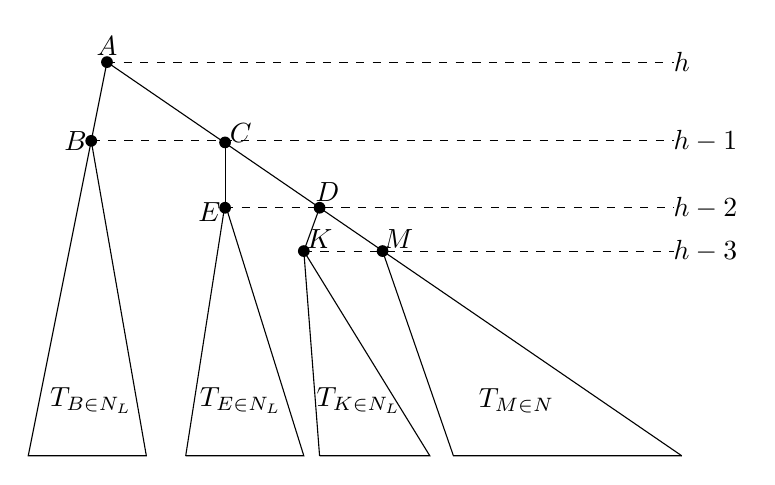
\begin{tikzpicture}

\draw(1.8,5.3) -- (9.1,0.3) ;
\draw(1.8,5.3) -- (0.8,0.3) -- (2.3,0.3) -- (1.6,4.3);
\draw (2.8,0.3) -- (4.3,0.3) -- (3.3, 3.5) -- (2.8,0.3);
\draw (4.5,0.3) -- (5.9,0.3) -- (4.3, 2.9) -- (4.5,0.3);
\draw (3.3, 3.5) -- (3.3, 4.28);
\draw (4.3, 2.9) -- (4.5, 3.45);
\draw  (9.1,0.3) -- (6.2,0.3) --  (5.3, 2.9);

\draw[dashed](1.8,5.3) -- (9,5.3) ;
\draw[dashed] (1.6,4.3) -- (9,4.3);
\draw[dashed] (3.3, 3.45) -- (9,3.45);
\draw[dashed] (4.3, 2.9) --  (9,2.9) ;

\node at (9.1,5.3) {$h$};
\node at (9.4,4.3) {$h-1$};
\node at (9.4,3.45) {$h-2$};
\node at (9.4,2.9) {$h-3$};

\node [circle, fill=black, inner sep = 1.5pt, minimum size=1pt] at (1.8,5.3) {};
\node [circle, fill=black, inner sep = 1.5pt, minimum size=1pt] at (1.6,4.3) {};
\node [circle, fill=black, inner sep = 1.5pt, minimum size=1pt] at (3.3, 4.28) {};
\node [circle, fill=black, inner sep = 1.5pt, minimum size=1pt] at (3.3, 3.45) {};
\node [circle, fill=black, inner sep = 1.5pt, minimum size=1pt] at (4.5, 3.45) {};
\node [circle, fill=black, inner sep = 1.5pt, minimum size=1pt] at (4.3, 2.9) {};
\node [circle, fill=black, inner sep = 1.5pt, minimum size=1pt] at (5.3, 2.9) {};

\node (start) at (1.8, 5.5) {$A$}; 
\node (first) at (1.4, 4.3) {$B$}; 
\node (firstr) at (3.5, 4.4) {$C$}; 
\node (second) at (3.1, 3.4) {$E$}; 
\node (secondr) at (4.6, 3.65) {$D$}; 
\node (third) at (4.5, 3.05) {$K$}; 
\node (thirdr) at (5.5, 3.05) {$M$}; 
\node (firstt) at (1.6, 1) {$T_{B \in N_L}$}; 
\node (firstt) at (3.5, 1) {$T_{E \in N_L}$}; 
\node (firstt) at (5, 1) {$T_{K \in N_L}$}; 
\node (firstt) at (7, 1) {$T_{M \in N}$}; 
\end{tikzpicture}
% Use the relevant command to insert your figure file.
% For example, with the graphicx package use
% figure caption is below the figure
\caption{A worst-case parse tree for superlinear grammar.}
\label{superlin}       % Give a unique label
\end{figure}

Applying Lemma \ref{thmetalin} and Corollary \ref{coldepth}, we deduce with the corollary.
\begin{corollary} 
Let  $G = (\Sigma, N, P)$ be a metalinear grammar and $D=(V, E, \Sigma)$ be a directed labelled graph with $n$ nodes. Then CFL-reachability problem for $G$ and $D$ is in $NC^2$.
\end{corollary}
\paragraph{Superlinear languages}
Let $G = (\Sigma, N, P)$ be a context-free grammar. $G$ is \textit{superlinear} if all productions of $P$ satisfy these conditions:
\begin{enumerate}
\item there is a subset $N_L \subseteq N$ such that every $A \in N_L$ has only linear productions $A\rightarrow aB$ or $A\rightarrow Ba$, where $B \in N_L$ and $a \in \Sigma$.
\item if $A \in N \setminus N_L$, then $A$ can have non-linear productions of the form $A \rightarrow BC$ where $B\in N_L$ and $C \in N$, or linear productions of the form $A\rightarrow \alpha B$ | $B \alpha$ | $\alpha$ for $B \in N_L$, $\alpha \in \Sigma^*$.
\end{enumerate}


It can be seen from conditions above, that superlinear grammars contain the metalinear grammars.
\begin{lemma}
\label{superlin}
Let  $G = (\Sigma, N, P)$ be a superlinear grammar and $D=(V, E, \Sigma)$ be a directed labelled graph with $n$ nodes. Then the length of the maximum in all nonterminals and all pairs of graph nodes shortest path labelled by a string from $L(G)$ ($\mathzapf{L}$) is $O(|N^2|n^4)$.
\end{lemma}
\begin{proof}
Let's construct a parse tree of maximum height $h$ from the root to leaves. Let $A$ be a nonterminal at the root of the parse tree $T_A$. We have two cases to consider:
\begin{enumerate}
\item  $A \in N_L$ or $A \in N \setminus N_L$ and $A$ has linear productions: then the tree with $A$ at the root is the same tree as parse tree for linear grammar and it has $O(h)$ leaves.
\item  $A \in N \setminus N_L$ and $A \rightarrow BC \in P$: then number of leaves in the tree $le(T_A)$ can be expressed with the following reccurent formula: $le(T_A) = le(T_B) + le(T_C) = h(T_B) + le(T_C) = h(T_A) - 1 + le(T_C)$.
\end{enumerate}
In the worst case, we have to add tree with $i$ leaves on every $i$-th level of the parse tree (counting from $h-1$ to 0) (see Figure \ref{superlin}). By Lemma  \ref{lem:treeheight}, $h \le |N|n^2$, so in the worst case the highest tree will have $|N|n^2-1 + |N|n^2 - 2 ... + 1 = O(|N^2|n^4)$ leaves.
\end{proof}


Combining Lemma \ref{superlin} and Corollary \ref{coldepth} we are able to conclude the following.
\begin{corollary} 
Let  $G = (\Sigma, N, P)$ be a superlinear grammar and $D=(V, E, \Sigma)$ be a directed labelled graph with $n$ nodes. Then CFL-reachability problem for $G$ and $D$ is in $NC^2$.
\end{corollary}

\subsection{Dyck languages}
\textit{Dyck language over $\Sigma_k$} is the set of well-balanced words over alphabet $\Sigma_k = \{(_1, (_2, ..., (_k, )_1, )_2, ..., )_k\}$. Dyck language can be defined by the following rules:
\\$S \rightarrow SS$ | $S \rightarrow \varepsilon$ |$S \rightarrow (_1S)_1$ | $S \rightarrow (_2S)_2$ | ... | $S \rightarrow (_kS)_k$, where $S$ is the start symbol, and $\varepsilon$ is the empty string. We will denote the Dyck language over $\Sigma_i$ by $D_i$.


Dyck languages play an important role in formal languages theory. The famous Chomsky-Sch\"utzenberger theorem states that every context-free language $L$ can be represented via a regular language $R$ and a Dyck language $D_n$, which are combined by means of an intersection and a homomorphism $h$. 
\begin{equation}
L = h(D_n \cap R)
\end{equation}


Because every context-free language can be represented with Dyck language, it is natural to expect that CFL-reachability is P-complete for Dyck languages. P-completeness for the similiar problem LGAP in case of $D_2$ was proved in \cite*{PCompl, LReach, Regularrealizability}. We will show that $\mathzapf{L}$ is exponential for $D_k$ where $k\ge2$, so our circuit is not effective in that case.
\begin{lemma}[Pierre]
\label{pierrelem}
The rational indexes of generators of context-free languages belongs to $exp(\Theta(n^2/\ln n))$.
\end{lemma}
\begin{theorem}
Let $L$ be a Dyck language over $k \ge 2$ brackets and $D=(V, E, \Sigma)$ be a directed labelled graph with $n$ nodes. Then, $\mathzapf{L}$  belongs to $exp(\Theta(n^2/\ln n))$.
\end{theorem}
\begin{proof}
By definition, generator is a context-free language which can transform into any context-free language through a rational transduction \cite{CFRat}.
Notice that for $k>2$ there is a homomorphism $g$ such that $D_k = g^{-1}(D_2)$ can be constructed. Thanks to the Chomsky-Sch\"utzenberger theorem, we have the following equation.
\begin{equation}
L = h(g^{-1}(D_2)\cap R)
\end{equation}
Thus, every context-free language can be generated by $D_k$, where $k \ge 2$. By \ref{pierrelem} we can conclude that $\mathzapf{L}$ for $D_k$ belongs to $exp(\Theta(n^2/\ln n))$. 
\end{proof}


We remark that strict upper bound on $\mathzapf{L}$ for arbitrary context-free grammar is obtained from Lemma \ref{pierrelem}, so it answers to the corresponding open question stated in \cite{HellingsCFPQ}.


It is known that $D_1$ is a generator of \textit{one-counter languages} \cite{GreibHier}. \textit{One-counter} languages are the languages recognized by \textit{one-counter automata} --- pushdown automata with a single stack symbol. For example, $L = \{w\#w'$ | $|w| \neq |w'|\}$ is one-counter language.



\begin{lemma}[Deleage, Pierre]
\label{dyck1lem}
The rational index of $D_1$ is in $O(n^2)$.
\end{lemma}
\begin{theorem}
\label{onecounter}
Let $L$ be a one-counter language, and $D=(V, E, \Sigma)$ be a directed labelled graph with $n$ nodes. Then, CFL-reachability problem for $L$ and $D$ is in $NC^2$.
\end{theorem}
\begin{proof} 
Because $D_1$ is a generator of one-counter languages \cite{GreibHier}, $D_1$ rationally dominates any one-counter language. If $L$ rationally dominates $L'$, then there exists an integer $c$ such that for every $n \in \mathbb{N}$ $\rho_{L'(n)} < cn(\rho_L(cn) + 1)$ \cite{RatBasic}.  Thus, the rational index of any one-counter language doesn't exceed $O(n^3)$, and by Corollary \ref{coldepth}, the depth of the circuit for one-counter languages is $O(\log^2 n)$.
\end{proof}


Notice that there is an effective sequential algorithm for CFL-reachability for $D_1$ based on matrix multiplication \cite{Bradford}. We believe that using Theorem \ref{onecounter} it can be extended for working with one-counter languages.

\subsection{Greibach languages and substitution closures}
Consider families of linear and one-counter languages. We can see that they are ``easy`` for CFL-reachability (Theorem \ref{onecounter}, Corollary \ref{linear}). One reason for this is that they are defined by natural restrictions on grammars or pushdown automatons (PDA). Restricting a PDA such that the height of its stack is only allowed to increase and then to decrease, thus performing only one turn, leads to the definition of one-turn PDAs. It is known that these PDAs can be characterized by linear grammars \cite{KUTRIB20072152}. One-counter languages are recognized by PDA with only one stack symbol. The same restrictions holds for substition closures of these languages, because substitution corresponds to a nesting of the pushdown stack \cite{Ginsburg1975}. It is easily observed that substitution closure of polinomially-bounded $\mathzapf{L}$ language yields polinomially-bounded $\mathzapf{L}$ language. 


But some of the restrictions on the pushdown store or on the grammar cannot be simulated by others. It is exactly the case of linear and one-counter languages: they and their iterated substitution closures are distinct families of context-free languages \cite{BEAUQUIER198191}.
Hierarchy of linear languages, one-counter languages and their substitution closures is illustrated in Figure \ref{hierarchy}. 


\begin{figure}
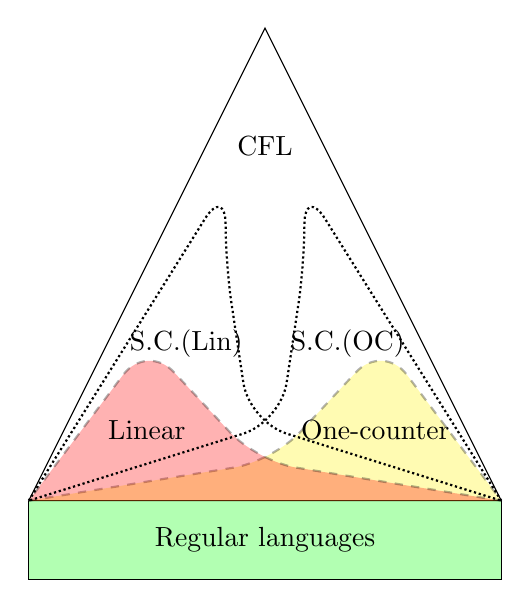
\begin{tikzpicture}
\draw[fill=green, opacity=0.3](0,1) -- (0,0) -- (6,0) --  (6,1);
\draw(0,1) -- (0,0) -- (6,0) --  (6,1);
\draw(0,1) -- (6,1) -- (3, 7) -- (0,1) ;
\draw[thick, dashed, rounded corners=5mm, fill=yellow, opacity=0.3] (0,1) -- (3.1, 1.5) -- (4.5, 3) -- (6,1);
\draw[thick, dashed, rounded corners=5mm, fill=red, opacity=0.3] (6,1) -- (2.9, 1.5) -- (1.5, 3) -- (0,1);
\draw[thick, densely dotted, rounded corners=5mm](0,1) -- (2.5, 5) -- (2.5,4)-- (2.8, 2) -- (6,1);
\draw[thick, densely dotted, rounded corners=5mm](6,1) -- (3.5, 5) -- (3.5,4)-- (3.2, 2) -- (0,1);

\node (reg) at (3, 0.5) {Regular languages}; 
\node (cfl) at (3, 5.5) {CFL}; 
\node (lin) at (1.5, 1.9) {Linear}; 
\node (one) at (4.4, 1.9) {One-counter}; 
\node (linsc) at (2, 3) {S.C.(Lin)}; 
\node (ocsc) at (4.05, 3) {S.C.(OC)}; 
\end{tikzpicture}
% Use the relevant command to insert your figure file.
% For example, with the graphicx package use
% figure caption is below the figure
\caption{A hierarchy of linear languages (Lin), one-counter languages (OC) and their substitution closures (S.C).}
\label{hierarchy}       % Give a unique label
\end{figure}
Family of \textit{Greibach languages} is the substitution closure of linear and one-counter languages. It is a large strict subfamily of the family of context-free languages: it does not contain the language $D_2$ \cite{Autebert1997}. Because it is the substitution closure of two polinomially-bounded $\mathzapf{L}$ languages, we have the following corollary.
\begin{corollary} 
Let  $L$ be a Greibach language and $D=(V, E, \Sigma)$ be a directed labelled graph with $n$ nodes. Then CFL-reachability problem for $L$ and $D$ is in $NC^2$.
\end{corollary}
